% I have removed Most of the comments for easy readability. You could
%look at the OG with modification doc for more info if needed. 



\documentclass[journal]{IEEEtran}
%

%\ifCLASSINFOpdf
  \usepackage{graphicx, soul}
  % declare the path(s) where your graphic files are
  % \graphicspath{{../pdf/}{../jpeg/}}
  % and their extensions so you won't have to specify these with
  % every instance of \includegraphics
  % \DeclareGraphicsExtensions{.pdf,.jpeg,.png}
%\else
  % or other class option (dvipsone, dvipdf, if not using dvips). graphicx
  % will default to the driver specified in the system graphics.cfg if no
  % driver is specified.
  % \usepackage[dvips]{graphicx}
  % declare the path(s) where your graphic files are
  % \graphicspath{{../eps/}}
  % and their extensions so you won't have to specify these with
  % every instance of \includegraphics
  % \DeclareGraphicsExtensions{.eps}
%\fi



% correct bad hyphenation here
% \hyphenation{op-tical net-works semi-conduc-tor}


\begin{document}
%
% paper title
% Titles are generally capitalized except for words such as a, an, and, as,
% at, but, by, for, in, nor, of, on, or, the, to and up, which are usually
% not capitalized unless they are the first or last word of the title.
% Linebreaks \\ can be used within to get better formatting as desired.
% Do not put math or special symbols in the title.
\title{ A Fruitful Attempt at Image Classification \\ }


\author{Group 28: Roan Gibbons, Aleksas Kliska, Josh Cottrell, Rhys Milling, Scott Clark, Jonathan Hayter}




% The paper headers
\markboth{Intelligent Systems 2 - Group project}%
{Shell \MakeLowercase{\textit{et al.}}: Bare Demo of IEEEtran.cls for IEEE Journals}




% make the title area
\maketitle

% As a general rule, do not put math, special symbols or citations
% in the abstract or keywords.
\begin{abstract}
In computer science, there are few faster-growing disciplines than Machine Learning (ML). One such area of ML that has made large strides in recent years is image classification, in which a computer can classify a given image into a set of classes. Our goal in this paper is to construct and train a Convolutional Neural Network (CNN) against the CIFAR-10 dataset so that it can accurately classify images out of 10 possible classes. To do this we will be using the Tensorflow 2 library in a Python 3 environment, this will efficiently handle the structuring of the CNN and its optimization. We have run the model 10 times and taken an average to account for outliers. On the validation set, we have achieved an average classification test error of 12.60\%, with all test errors falling in the range between 12.40\% and 12.88\%, and an average test loss of 0.4606.\end{abstract}


\IEEEpeerreviewmaketitle

\section{Introduction}

\IEEEPARstart{T}{he} task is to create
% You must have at least 2 lines in the paragraph with the drop letter
% (should never be an issue)
a machine learning model that can classify the 60000 images from the CIFAR-10 dataset [1] into a set of pre-defined categories. Historically, the task of image classification has been tackled with mostly traditional machine learning approaches. More recently, however, beginning in 2012 with Krizhevsky’s AlexNet [2], a new, deep learning approach has been found to be more successful at classifying images. Typically, CNNs are used for this task, these are multi-layer neural networks that are trained with a back-propagation algorithm. In 2017, an accuracy of 95\% was achieved by 29 of the 38 teams entered into that year’s ImageNet competition, using similar methods to those used in AlexNet [3]. Computer vision is an important machine learning problem as it has countless applications such as medical imaging, object recognition and vision biometrics. It can be used to greatly enhance the safety and everyday lives of regular people. To try and solve this problem, we aimed to create a robust ML model that would be able to classify the images in the CIFAR-10 dataset using the Tensorflow library [4].


\section{Method}

The network we created is formed of 3 distinctly structured blocks, followed by a fully connected layer before an output layer. Each block contains two convolutional layers interspersed with batch normalisation layers, followed then by a max-pooling layer and finally a dropout layer to help avoid over-fitting. The convolutional layers are used primarily as a way of extracting features from the input data. Stacking convolutional layers as we have with smaller kernel sizes allows for a higher effective receptive field with fewer parameters than the alternative of one layer with a large filter. Besides keeping the number of parameters low, this approach also allows for greater non-linearity due to the addition of extra depth to the network, overall making the model more discriminative. Before passing the images into our model, they were first pre-processed. This involved normalizing the colour values of each pixel in all the images to a value between 0 and 1, it was then passed into the model.\par
As this model is quite deep, training it runs into the challenge of internal covariate shift, which dictates that as the ranges of the outputs for each layer change over the course of training, due to the altering of the weights and thus the magnitude of the resulting activation's, the training of the model becomes much slower as the subsequent layers must react to this differing input. [5] describes a method called 'batch normalisation' that helps to combat this by normalising the inputs at each stage. The max pooling layer in the block is used to reduce the size of the input to all subsequent layers. This helps to reduce the computational load by reducing the number of required parameters in the network. Dropout layers are a method of regularisation that avoids over-fitting by randomly 'dropping' a specific percentage of the neurons for a layer [6]. This is only relevant for the training examples as dropout layers are inactive once training is complete. Dropout forces the model not to simply memorize the training data and allows the network to be more resilient to over-fitting. We also apply the ridge regression technique (L2 regularisation) as a further method to avoid over-fitting which uses the square sum of the weights of the network as a regularisation constant.\par
As an activation function for each convolutional layer, we are using rectified linear units (ReLU) as this is a standard for deep learning. The alternative of the sigmoid function runs into the issue of vanishing gradients. As the sigmoid function has values between -1 and 1, the magnitude of the partial derivative of the cost function with respect to the weights decreases exponentially for neurons at the earlier layers of the network, due to the backpropogation algorithm multiplying a number of these small activations together. ReLU avoids this problem by having a range greater than or equal to zero. We also apply the Softmax activation function to the final layer of the network in order to explicitly convert the output into a vector of probabilities. Finally, we have utilised a categorical cross entropy loss function. This compares each predicted class probability to the actual desired output, 0 or 1, and subsequently calculates a loss based on how far the logarithm of the Softmax probability is from the desired value. As this loss is logarithmic in nature it creates a large loss for differences closer to 1 and a small loss for differences closer to 0. The formula for cross entropy loss is as follows:

\[L_{CE} = - \sum_{i=1}^{n} t_i \log {(p_i)}\textrm{, for n classes,} \]where \(t_i\) is the expected value and \(p_i\) is the Softmax probability for the \(i^{th}\) class.


\fontsize{9pt}{11pt}{
    \begin{figure*}[t!]
      %\resizebox{\linewidth}{!}{
      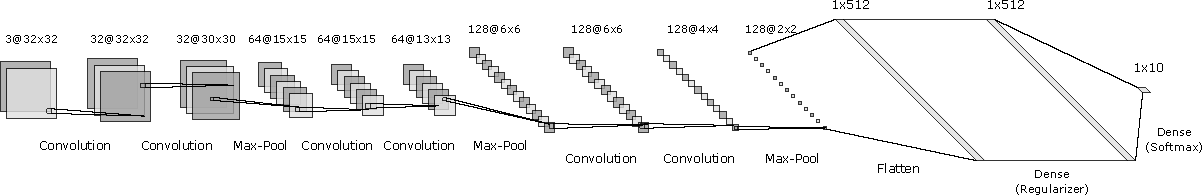
\includegraphics[width=\linewidth]{nn_final.pdf}
      %}
      \caption{Diagram of the Neural Network Model, annotated with layer type, and the size of the tensor at each stage, in the form of \emph{depth}@\emph{height}x\emph{width}}
    \end{figure*}
}


\section{Results \& Evaluation}

% Maybe move hardware bit to bottom of section now??
Training took place in a Python 3 environment on Google Colab, and their Compute Engine backend (GPU), this allowed us to train our model on an Nvidia Tesla K80 GPU and took around 51 minutes to complete. We measured two variables; test loss, test accuracy, and calculated test error. Test loss is an interpretation of how well the model is performing, lower is better. It is most helpful during training as it allows the model to train the network variables to allow improvements between epochs. Secondly, the test accuracy, is a comparison from the models predictions and the true data, letting us see how the model performed overall, the higher the better. Finally, we calculated our classification test error by using the formula \( test\ error = 1 - test\ accuracy\).

% Do we need Test Error since it's based off of test accuracy? Although we do run a small table then but there isn't much else to say - Rhys
% Only reason it is included is because in the assessment paper itself, it doesn't refer to accuracy, but rather test error - JJ

\begin{center}
  \begin{tabular}{c|c|c|c} 
    %\hline
    Run & Test Loss & Test Error & Test Accuracy \\ [0.5ex] 
    \hline
    1 & 0.4521 & 12.41\% & 87.59\% \\ 
    %\hline
    2 & 0.4639 & 12.65\% & 87.35\% \\
    %\hline
    3 & 0.4595 & 12.88\% & 87.12\% \\
    %\hline
    4 & 0.4596 & 12.69\% & 87.31\% \\
    %\hline
    5 & 0.4535 & 12.42\% & 87.58\% \\
    %\hline
    6 & 0.4680 & 12.69\% & 87.31\% \\
    %\hline
    7 & 0.4597 & 12.68\% & 87.32\% \\
    %\hline
    8 & 0.4508 & 12.40\% & 87.60\% \\
    %\hline
    9 & 0.4714 & 12.68\% & 87.32\% \\
    %\hline
    10 & 0.4680 & 12.47\% & 87.53\% \\ 
    %\hline
    Average & 0.4606 & 12.60\% & 87.40\% \\ [0.5ex]
  \end{tabular}
\end{center}

As can be seen in the table above, we ran our model a total of  10  times  in  order  to  take  an  average  of  accuracy  and  test loss, this was done to avoid the possibility of outliers affecting our data. It can be said that our model is accurate, achieving a test error just 7.5\% above most current state of the art systems. Training runs for 300 epochs, this number was chosen to ensure we could run the algorithm relatively quickly to iterate upon and still reach a peak in our test accuracy where more epochs would not necessarily cause much improvement. Our chosen optimisation algorithm was stochastic gradient descent (SGD) with momentum, as it is a standard in the field and the most familiar to us from our lectures and research. We chose to use this over regular gradient descent as SGD uses approximations in order to converge faster, allowing us to experiment with variables more often. It used a learning rate of 0.001, as we found the small step size prevented us from skipping a minimum; and a momentum of 0.9, in the hope that  it  would  lead  to  faster  converging and thus offset the disadvantage of the low learning rate. Our classification test error had an average of 12.60\%, which means that of the 10000 test images, our model misclassified just 1260 of them on average.

% Reading the VLE, it might be worthwhile including the configuration of each layer. - Rhys

\section{Conclusion \& Further Work}

Our network was able to achieve an average accuracy of 87.40\% on unseen data, not only was it able to achieve a high degree of accuracy, but it was able to do so consistently and reliably, with a range of less than 0.5\% over 10 runs. \par
The test loss of our model ceased to decrease at around the 150 epoch mark, this meant that there was little improvement in test accuracy from that point onward. Therefore, in order to rectify this problem, we'd implement an early stopping callback into our model in order to reduce time wasted for the algorithm to complete. Furthermore, our model used simple random initialization to set the commencing values of the weights and biases of the network which, combined with our use of stochastic gradient descent, means that our model has a random chance of finding a good minimum loss. We would point to the work of He et al. [7] as a way of testing the effect that more deliberate initialization techniques have on both the final accuracy of the network and the speed of training.


\ifCLASSOPTIONcaptionsoff
  \newpage
\fi



\begin{thebibliography}{1}

% ||||||||||||||||||||||||||||||||||||||||||||||||||||||||||||
% For syntax follow example below. Week 11 Latex video 12:00
%|||||||||||||||||||||||||||||||||||||||||||||||||||||||||||||

% Maybe sort out the link that is too long
\bibitem{}
A. Krizhevsky, V. Nair, G. Hinton, "CIFAR-10 Dataset", [Online] Available:
\emph{https://www.cs.toronto.edu/~kriz/cifar.html}

\bibitem{ImageNet Classification with Deep Convolutional
Neural Networks}
A. Krizhevsky, I. Sutskever and G. Hinton, \emph{"ImageNet Classification with Deep Convolutional Neural Networks"}, Papers.neurips.cc, 2012. [Online]. Available: \emph{https://papers.nips.cc/paper/2012/file/c399862d3b9d6b76c8436e924a68c45b-Paper.pdf}. %[Accessed: 28- Apr- 2021].

\bibitem{The Quartz guide to artificial intelligence: What is it, why is it important, and should we be afraid?}
D. Gershgorn, "The Quartz guide to artificial intelligence: What is it, why is it important, and should we be afraid?", \emph{Quartz}, 2017. [Online]. Available: \emph{https://qz.com/1046350/the-quartz-guide-to-artificial-intelligence-what-is-it-why-is-it-important-and-should-we-be-afraid/}. %[Accessed: 28- Apr- 2021].

\bibitem{}
Google LLC, "Tensorflow", [Online] Available:
\emph{https://www.tensorflow.org/}

\bibitem{Batch Normalization: Accelerating Deep Network Training by Reducing Internal Covariate Shift}
S. Ioffe, C. Szegedy, "Batch Normalization: Accelerating Deep Network Training by Reducing Internal Covariate Shift", \emph{ArXiv}, 2015. [Online]. Available: \emph{https://arxiv.org/abs/1502.03167}.

\bibitem{Dropout: A Simple Way to Prevent Neural Networks from Overfitting}
N. Srivastava, G. Hinton, A. Krizhevsky, I. Sutskeverm, R. Salakhutdinov, "Dropout: A Simple Way to Prevent Neural Networks from Overfitting", \emph{Journal of Machine Learning Research}, 2014. [Online]. Available: \emph{https://jmlr.org/papers/v15/srivastava14a.html}.

\bibitem{Delving Deep into Rectifiers: Surpassing Human-Level Performance on ImageNet Classification}
K. He, X. Zhang, S. Ren, J. Sun, "Delving Deep into Rectifiers: Surpassing Human-Level Performance on ImageNet Classification", \emph{ArXiv}, 2015. [Online]. Available: \emph{https://arxiv.org/abs/1502.01852}.

\end{thebibliography}


\end{document}


